\subsection{Optimization for the rectangular
scenario}\label{subsec:rectoptimization}

As in other scenarios, we have run a full factorial analysis, with low values of
each parameter, in order to identify the minimum values required to reach the
coverage. The complete analysis can be found in \code{coverage.ipynb}. The
configuration used is named ``RectangularCoverage''. We have found out that to
reach at least the \(99\%\) of the coverage, we need to have a broadcast radius
of at least \(7m\), the same of the high density scenario, but we also need
higher values for \(m\) and \(D\). If we use \(R\!=\!8m\) we get better results
for the other parameters. In particular, we have found the following minimum
configuration the we consider ``good'' and ``well balanced'' since it does not
use the value \code{1} for any of the parameters. So for the coverage the
situation is the same for a square or a rectangle.

\begin{center}
	\begin{tabular}{cccc}
		\toprule
		R & T & m & \(\max(\delta)\) \\
		\midrule
		\(8m\) & \(2s\) & \(2\,\mathit{copies}\) & \(2s\) \\
		\bottomrule
	\end{tabular}
\end{center}

As in the other scenarios, to optimize the \standout{total broadcast time} we
need to increase the broadcast radius (with higher energy consumption) or
decrease the size of the hear window. The results are in the file
\code{broadcast-time.ipynb}. The configuration used is named
``RectangularTime'', where we use, as suggested from the plots of
\code{2kr.ipynb}, high values for \(m\) and low value for the maximum relay
delay. As shown in \figref{fig:recttimeff}, also in this case a low \(T\)
reduces a lot the broadcast time.

\begin{figure}[hbt]
	\centering
	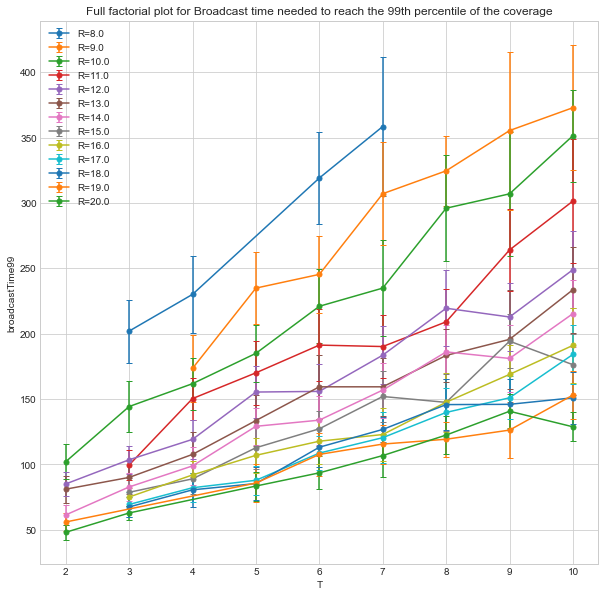
\includegraphics[width=0.6\textwidth]{img/rect/broadcasttime-T-ffplot.png}
	\caption{The broadcast time is lower with higher values of the broadcast
	radius and lower values of the size of the hear window (95\% confidence
	intervals)}\label{fig:recttimeff}
\end{figure}

We note that the broadcast time is usually higher compared to the results of the
high density scenario: this is due to the fact that in the case of a square
floorlan, the message is relayed radially in all the directions and it reaches
the extremes of the floorplan more or less at the same time. In the rectangular
case, since a dimension is much longer than the other, the message need to hop
through an higher number of users in order to reach the extremes in the longer
dimension.

To optimize the \standout{energy efficiency}, we have studied the number of
messages. Factorial analysis is available in \code{messages.ipynb}. We use low
values for the broadcast radius (that obviously improves energy efficiency). The
configuration used is named ``RectangularMessages''.

As we can see from \figref{fig:rectmessagesff}, we get that, as in the other
scenarios, the maximum number of copies hugely affects the total number of
messages sent, as previously found by the \(2^{k}r\) analysis. Also increase the
size of the hear window have benefits.

\begin{figure}[htb]
	\centering
	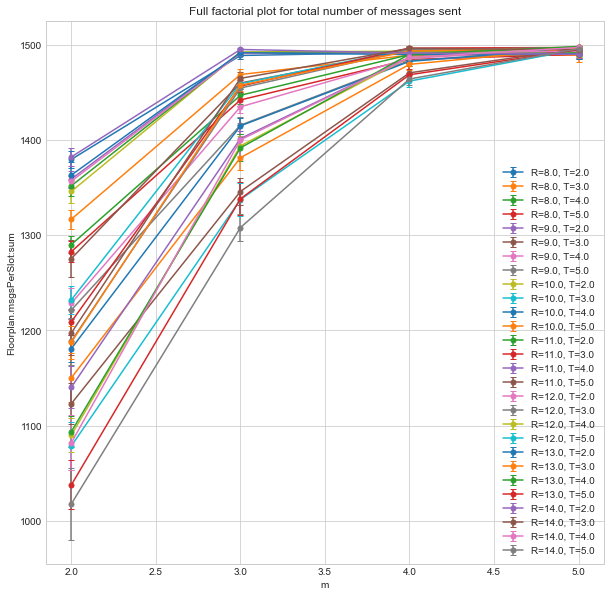
\includegraphics[width=0.6\textwidth]{img/rect/messages-m-ffplot.png}
	\caption{With low values of the maximum number of copies and higher
	values for the size of the hear window, we get a lower number of
	messages sent}\label{fig:rectmessagesff}
\end{figure}

So, we can improve energy efficiency with the same parameter manipulation of
other scenarios, taking into consideration the trade-off between broadcast time
and energy consumption regarding the hear window.

For the \standout{total number of collisions}, we can reduce it by reducing the
broadcast radius and the maximum number of copies. Also helps increasing the
maximum relay delay, like in the other scenarios. Factorial analysis with the
\(m\) and \(\max(\delta)\) parameters is available in \code{collisions.ipynb},
using the configuration named ``RectangularCollisions''.

\figref{fig:rectcollisionsff} shows the results.  Also in this case, \(m\!=\!2\)
is a good setup because of trickle relaying algorithm.

\begin{figure}
	\centering
	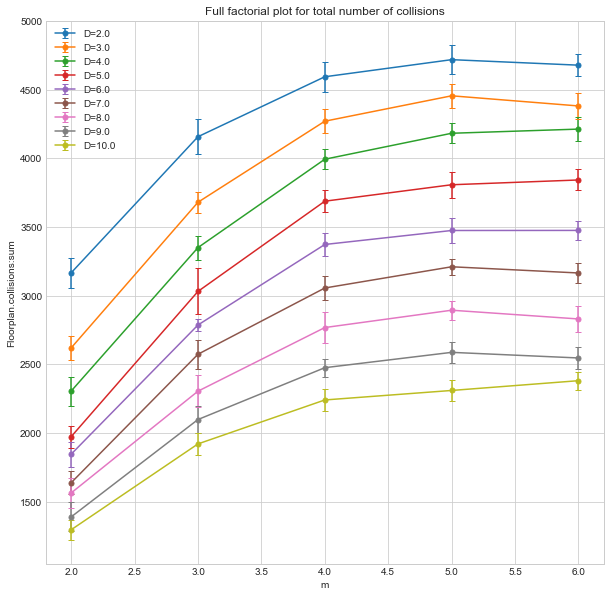
\includegraphics[width=\textwidth]{img/rect/collisions-m-ffplot.png}
	\caption{The number of collisions is inverse linearly dependent on the
	maximum	relay delay}\label{fig:rectcollisionsff}
\end{figure}

\subsubsection{Conclusions}\label{subsubsec:rectconclusions}

\begin{itemize}
	\item The minimal configuration to get a nearly perfect coverage is with
		\(R\!=\!8m\), \(T\!=\!2s\), \(m\!=\!2\) and
		\(\max(\delta)\!=\!2s\). Higher values for these parameters does
		not break the coverage.
	\item The fact that the floorplan is rectangular does not affect a lot
		the performance indexes we have studied, except for the
		broadcast time that gives higher values.
\end{itemize}
